\global\long\def\veraw#1#2#3{#1\models_{#2}#3}


\global\long\def\vera#1#2{#1\models#2}


\global\long\def\nonvera#1#2{#1\nvDash#2}


\global\long\def\nonveraw#1#2#3{#1\nvDash_{#2}#3}


\global\long\def\verita#1#2{#1\in V(#2)}


\global\long\def\entail#1#2{#1\models#2}


\global\long\def\semantica#1#2#3{#1\vdash_{#2}#3}


\global\long\def\semGen#1#2{#1\vdash#2}


\global\long\def\boxx#1{\square#1}


\global\long\def\diam#1{\diamond#1}


\global\long\def\dia{\diamond a}


\global\long\def\boa{\boxx a}


\global\long\def\forhten#1#2#3{\forall#1#2\Rightarrow#3}


\global\long\def\implica#1#2{#1\Rightarrow#2}



\chapter{Introduction}

$a$ è vera nel mondo $\alpha$, e scriviamo $\mu\models_{\alpha}a$

se 
\begin{itemize}
\item $a$ è una lettera enunciativa allora deve valere $\verita a{\alpha}$ 
\item $a$ è del tipo: $a\lor b$ .... allora.... $\mu\models_{\alpha}a$
oppure $\mu\models_{\alpha}b$ 
\end{itemize}

\section{Formule di Logica modale e significato}

\subsection{Relazione seriale}

Ip) Frame F con relazione R seriale

Ts) $\boa\implies\dia$

Dimostrazione:

Se non vale: $\veraw{\mu}{\alpha}{\boa}$ allora immediatemente si
ha la tesi in quanto l'antecedente è falso.

Se invce: $\veraw{\mu}{\alpha}{\boa}$ allora

$\forhten{\beta}{\,:\,\alpha R\beta}{\veraw{\mu}{\beta}a}$ per definizione
di box, 

inoltre dato che R seriale per Ip si ha anche che $\exists\beta:\:(\alpha,\beta)\:\in R$ 

da cui: $\veraw{\mu}{\alpha}{\dia}$ per definizione di diamond (esiste
$\beta$ in relazione con $\alpha$ per la serialità e in $\alpha$
vale $a$ dato che $\veraw{\mu}{\alpha}{\boa}$ )\\

		

Ip) $\boa\implies\dia$

Ts) Frame F con relazione R seriale

\begin{center} 
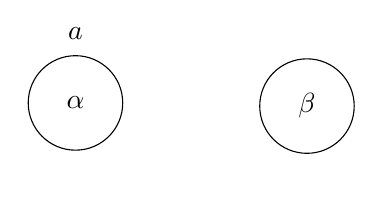
\begin{tikzpicture}[scale=0.2] 
\tikzstyle{every node}+=[inner sep=0pt] 
\draw [black] (24.2,-13) circle (3);
\draw (24.2,-13) node {$\alpha$};

\draw (24.2,-8.6) node {$\boxx{a}$};
\draw [black] (38.9,-13.2) circle (3);
\draw (38.9,-13.2) node {$\beta$}; 

\draw (24,-17.3) node {\sout{$\dia$}};   %%diamond a sbarrato
\end{tikzpicture} \end{center}

Per assurdo:

Suppongo di trovarmi in un mondo come quello in figura (wow) in cui
\mbox{$\veraw{\mu}{\alpha}{\boa}$ }, e suppongo che la relazione
R del frame NON sia seriale cioè $\sim\exists\beta:(\alpha R\beta)$,
se è così vale sicuramente $\veraw{\mu}a{\boa}$ (dato che $\alpha$
non ha successori) , d'altra parte per come è il mondo considerato,
cioè si nega la tesi, assurdo\sout{.} 

\subsection{Relazione simmetrica}

Ip) R simmetrica

Ts) $a\implies\boxx{\dia}$

Suppongo che $\veraw{\mu}{\alpha}a$ (se no avrei già la tesi), due
casi:

\textbf{Caso 1}: Da $\alpha$ non parte nessun arco, allora sicuramente
$\veraw{\mu}{\alpha}{\boxx x}$ con $x$ qualsiasi e in particolare
$\veraw{\mu}{\alpha}{\boxx{\dia}}$

\begin{center} 
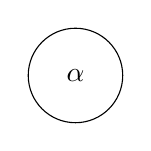
\begin{tikzpicture}[scale=0.2] 
\tikzstyle{every node}+=[inner sep=0pt] 

\draw [black] (24.2,-13) circle (3);
\draw (24.2,-13) node {$\alpha$};

\end{tikzpicture} \end{center}

\textbf{Caso 2}: Esiste almeno un $\beta$ tale che $\alpha R\beta$.

\begin{center} 
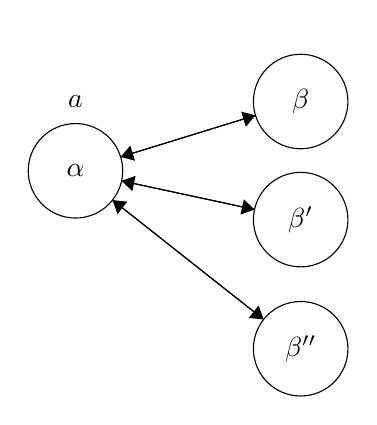
\begin{tikzpicture}[scale=0.2]
\tikzstyle{every node}+=[inner sep=0pt]
\draw [black] (24.2,-12.7) circle (3);
\draw (24.2,-12.7) node {$\alpha$};

\draw (24.2,-8.3) node {$a$}; 
\draw [black] (38.5,-8.3) circle (3); 
\draw (38.5,-8.3) node {$\beta$}; 
\draw [black] (38.5,-15.8) circle (3); 
\draw (38.5,-15.8) node {$\beta'$}; 
\draw [black] (38.5,-24) circle (3); 
\draw (38.5,-24) node {$\beta''$}; 

\draw (38.5,-3.7) node {$\dia$};

\draw (38.5,-11.7) node {$\dia$}; 
\draw (38.5,-20.2) node {$\dia$}; 

\draw [black] (27.07,-11.82) -- (35.63,-9.18);
\fill [black] (35.63,-9.18) -- (34.72,-8.94) -- (35.02,-9.9); 
\draw [black] (35.63,-9.18) -- (27.07,-11.82); 
\fill [black] (27.07,-11.82) -- (27.98,-12.06) -- (27.68,-11.1);
\draw [black] (27.13,-13.34) -- (35.57,-15.16);
\fill [black] (35.57,-15.16) -- (34.89,-14.51) -- (34.68,-15.48);
\draw [black] (35.57,-15.16) -- (27.13,-13.34); 
\fill [black] (27.13,-13.34) -- (27.81,-13.99) -- (28.02,-13.02); 
\draw [black] (26.55,-14.56) -- (36.15,-22.14);
\fill [black] (36.15,-22.14) -- (35.83,-21.25) -- (35.21,-22.04); 
\draw [black] (36.15,-22.14) -- (26.55,-14.56); 
\fill [black] (26.55,-14.56) -- (26.87,-15.45) -- (27.49,-14.66);
\end{tikzpicture} \end{center}

Dato che la relazione è simmetrica se $\alpha R\beta$ allora \textbf{$\beta R\alpha$.}
Dato che $\veraw{\mu}{\alpha}a,$ in ognuno di questi $\beta$, $\beta'$,$\beta''$
ecc. vale $\dia$ perché ognuno di loro è in relazione con $\alpha$. 

Allora per ognuno di questi $\beta$ si ha $\veraw{\mu}{\beta}{\dia}$,
(esiste infatti un mondo, $\alpha$, in cui vale $a$) da cui: $\veraw{\mu}{\alpha}{\boxx{\dia}}$
\\

Ip) $a\implies\boxx{\dia}$

Ts) R simmetrica

Per assurdo:

suppongo R non sia simmetrica e considero un frame con soli $\alpha$
e $\beta$ e in cui $R=\{(\alpha,\beta)\}$ . In questo frame considero
un modello con funzione di verità tale che: $V(A)=\{\alpha\}$.

In $\beta$ non vale $\dia$ perché $\beta$ non è in relazione con
nessun mondo, per questo: $\nonveraw{\mu}{\alpha}{\boxx{\dia}}$

\begin{center} 
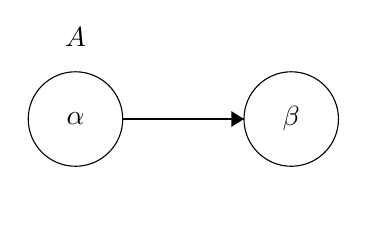
\begin{tikzpicture}[scale=0.2] \tikzstyle{every node}+=[inner sep=0pt] 
\draw [black] (24.2,-12.7) circle (3); 
\draw (24.2,-12.7) node {$\alpha$}; 

\draw (24.2,-7.5) node {$A$};

\draw [black] (37.9,-12.7) circle (3);
\draw (37.9,-12.7) node {$\beta$};


\draw (37.9,-7.5) node {\sout{$\dia$}}; 

\draw (24.2,-17.8) node {\sout{$\boxx{\dia}$}}; 

\draw [black] (27.2,-12.7) -- (34.9,-12.7);
\fill [black] (34.9,-12.7) -- (34.1,-12.2) -- (34.1,-13.2); 
\end{tikzpicture} \end{center}

$ $

\subsection{Funzione parziale}

\begin{tabular}{|c|c|c|}
\hline 
$\diam{}{a\Rightarrow}\boxx a$  & funzione parziale  & $\forhten{\alpha}{:\,\alpha R\beta,\:\beta R\gamma}{\beta}=\gamma$\tabularnewline
\hline 
\end{tabular}

Funzione parziale, dimostrazione

.

Ip) funzione parziale

Ts) $\diam{}{a\Rightarrow}\boxx a$

.

$\diam{}a$ falsa allora dato che l'antecedente è falso di ha $\implica{\diam{}a}{\boxx a}$

$\diam{}a$ vera allora $\exists\beta$:$\alpha R\beta$ e$\in V(\beta)$,
ma dato che la funzione è parziale questo $\beta$ è unico !

da cui $\vera{\mu}{\implica{\diamond a}{\boxx a}}$

.

.

Ip) $\diam{}{a\Rightarrow}\boxx a$

Ts) funzione parziale

.

.

Per assurdo: suppongo non che la funzione non sia parziale. Se è così
$\exists\alpha:$ $\alpha R\beta,$ $\alpha R\gamma$, considero un
modello in cui V(A) = \{$\beta$ \} , $\boxx A$ non vale in $\alpha$
dato che A è falsa in $\gamma$, il che contraddice l'ipotesi (BAM!)\\
\\
\subsection{Funzione totale}

\begin{tabular}{|c|c|c|}
\hline 
$\diam{}{a\iff}\boxx a$  & funzione totale  & $\forall\alpha\exists\,!\,\beta:\:\alpha R\beta$ \tabularnewline
\hline 
\end{tabular}\\
\\


non ci sono ``conti'' da fare, R è seriale sse R è seriale $\boxx a\implies\diam a$
, e se R è una funzione parziale $\implica{\diam a}{\boxx a}$

quindi dato che l'implica prevede un and di implica da una parte e
dall'altra per definizione abbiamo la tesi

.

\subsection{Relazione euclidea}

\begin{tabular}{|c|c|c|}
\hline 
$\diam{}{a\Rightarrow}\boxx{\diam a}$  & relazione euclidea  & $\forhten{\alpha,\beta,\gamma}{:\:(\alpha R\beta,\:\alpha R\gamma)}{\beta}R\gamma$
da cui anche: $\beta$R$\beta$, $\gamma R\gamma$, $\gamma$R$\beta$\tabularnewline
\hline 
\end{tabular}\\
\\


Ip) relazione euclidea

Ts) $\diam{}{a\Rightarrow}\boxx{\diam a}$

Suppongo sia vero l'antecedente (se falso ho finito), quindi vale:
$\dia$ da cui: $\vera{\mu}{\dia}$

dato che $\dia$ si ha che esiste almeno un $\beta$ tale che in beta
vale a

solo un beta: autoanello perché euclidea e quindi $\boxx{\dia}$

diversi beta: ognuno dei vari $\beta'$, $\beta''$ , ecc. sono in
relazione con $\beta$, dato che la relazione è euclidea, pertanto
dato che in $\beta$ vale $a$, in ognuno di loro vale $\dia$ \\


\begin{center} 
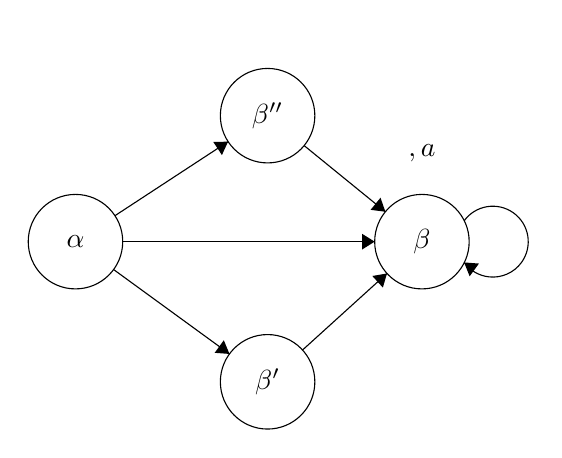
\begin{tikzpicture}[scale=0.2] 
\tikzstyle{every node}+=[inner sep=0pt]
\draw [black] (24.5,-18.4) circle (3);
\draw (24.5,-18.4) node {$\alpha$};
\draw [black] (46.5,-18.4) circle (3); 
\draw (46.5,-18.4) node {$\beta$};
\draw [black] (36.7,-27.3) circle (3); 
\draw (36.7,-27.3) node {$\beta'$};
\draw (23.9,-12.8) node {$\dia$};
\draw (46.5,-12.8) node {$\dia, a$};
\draw (36.7,-22.1) node {$\dia$};
\draw [black] (36.7,-10.4) circle (3);
\draw (36.7,-10.4) node {$\beta''$};
\draw (36.7,-4.9) node {$\dia$};
\draw [black] (27.5,-18.4) -- (43.5,-18.4); 
\fill [black] (43.5,-18.4) -- (42.7,-17.9) -- (42.7,-18.9);
\draw [black] (26.92,-20.17) -- (34.28,-25.53); 
\fill [black] (34.28,-25.53) -- (33.92,-24.66) -- (33.34,-25.46); 
\draw [black] (27.01,-16.75) -- (34.19,-12.05); 
\fill [black] (34.19,-12.05) -- (33.25,-12.07) -- (33.8,-12.9); 
\draw [black] (49.18,-17.077) arc (144:-144:2.25);
\fill [black] (49.18,-19.72) -- (49.53,-20.6) -- (50.12,-19.79);
\draw [black] (39.02,-12.3) -- (44.18,-16.5);
\fill [black] (44.18,-16.5) -- (43.87,-15.61) -- (43.24,-16.38);
\draw [black] (38.92,-25.28) -- (44.28,-20.42);
\fill [black] (44.28,-20.42) -- (43.35,-20.58) -- (44.02,-21.32); 
\end{tikzpicture}
\end{center} 

Ip)$\diam{}{a\Rightarrow}\boxx{\diam a}$

Ts) relazione euclidea

Per assurdo, suppondo valga ip) ma non la tesi

Considero un Frame in cui: $\alpha R\beta,$ $\alpha R\gamma,$ $\beta R\gamma$
ma NON $\beta R\gamma$ cioè si ha un frammento in cui non vale l'euclidea.
Poniamo che il modello sia tale che $V(A)$$=\{\gamma\}$

In queste ipotesi vale $\dia$ dato che in $\gamma$ vale $a$. In
$\beta$ non vale $a$ e neppure $\dia$ perché non ha ``uscite'',
da cui in $a$ non vale $\boxx{\dia}$ contraddicendo così l'ipotesi
(BAM!) \\
\\

